% GNUPLOT: LaTeX picture with Postscript
\begingroup
  % Encoding inside the plot.  In the header of your document, this encoding
  % should to defined, e.g., by using
  % \usepackage[latin1,<other encodings>]{inputenc}
  \inputencoding{latin1}%
  \makeatletter
  \providecommand\color[2][]{%
    \GenericError{(gnuplot) \space\space\space\@spaces}{%
      Package color not loaded in conjunction with
      terminal option `colourtext'%
    }{See the gnuplot documentation for explanation.%
    }{Either use 'blacktext' in gnuplot or load the package
      color.sty in LaTeX.}%
    \renewcommand\color[2][]{}%
  }%
  \providecommand\includegraphics[2][]{%
    \GenericError{(gnuplot) \space\space\space\@spaces}{%
      Package graphicx or graphics not loaded%
    }{See the gnuplot documentation for explanation.%
    }{The gnuplot epslatex terminal needs graphicx.sty or graphics.sty.}%
    \renewcommand\includegraphics[2][]{}%
  }%
  \providecommand\rotatebox[2]{#2}%
  \@ifundefined{ifGPcolor}{%
    \newif\ifGPcolor
    \GPcolortrue
  }{}%
  \@ifundefined{ifGPblacktext}{%
    \newif\ifGPblacktext
    \GPblacktexttrue
  }{}%
  % define a \g@addto@macro without @ in the name:
  \let\gplgaddtomacro\g@addto@macro
  % define empty templates for all commands taking text:
  \gdef\gplbacktext{}%
  \gdef\gplfronttext{}%
  \makeatother
  \ifGPblacktext
    % no textcolor at all
    \def\colorrgb#1{}%
    \def\colorgray#1{}%
  \else
    % gray or color?
    \ifGPcolor
      \def\colorrgb#1{\color[rgb]{#1}}%
      \def\colorgray#1{\color[gray]{#1}}%
      \expandafter\def\csname LTw\endcsname{\color{white}}%
      \expandafter\def\csname LTb\endcsname{\color{black}}%
      \expandafter\def\csname LTa\endcsname{\color{black}}%
      \expandafter\def\csname LT0\endcsname{\color[rgb]{1,0,0}}%
      \expandafter\def\csname LT1\endcsname{\color[rgb]{0,1,0}}%
      \expandafter\def\csname LT2\endcsname{\color[rgb]{0,0,1}}%
      \expandafter\def\csname LT3\endcsname{\color[rgb]{1,0,1}}%
      \expandafter\def\csname LT4\endcsname{\color[rgb]{0,1,1}}%
      \expandafter\def\csname LT5\endcsname{\color[rgb]{1,1,0}}%
      \expandafter\def\csname LT6\endcsname{\color[rgb]{0,0,0}}%
      \expandafter\def\csname LT7\endcsname{\color[rgb]{1,0.3,0}}%
      \expandafter\def\csname LT8\endcsname{\color[rgb]{0.5,0.5,0.5}}%
    \else
      % gray
      \def\colorrgb#1{\color{black}}%
      \def\colorgray#1{\color[gray]{#1}}%
      \expandafter\def\csname LTw\endcsname{\color{white}}%
      \expandafter\def\csname LTb\endcsname{\color{black}}%
      \expandafter\def\csname LTa\endcsname{\color{black}}%
      \expandafter\def\csname LT0\endcsname{\color{black}}%
      \expandafter\def\csname LT1\endcsname{\color{black}}%
      \expandafter\def\csname LT2\endcsname{\color{black}}%
      \expandafter\def\csname LT3\endcsname{\color{black}}%
      \expandafter\def\csname LT4\endcsname{\color{black}}%
      \expandafter\def\csname LT5\endcsname{\color{black}}%
      \expandafter\def\csname LT6\endcsname{\color{black}}%
      \expandafter\def\csname LT7\endcsname{\color{black}}%
      \expandafter\def\csname LT8\endcsname{\color{black}}%
    \fi
  \fi
    \setlength{\unitlength}{0.0500bp}%
    \ifx\gptboxheight\undefined%
      \newlength{\gptboxheight}%
      \newlength{\gptboxwidth}%
      \newsavebox{\gptboxtext}%
    \fi%
    \setlength{\fboxrule}{0.5pt}%
    \setlength{\fboxsep}{1pt}%
\begin{picture}(7200.00,4320.00)%
    \gplgaddtomacro\gplbacktext{%
      \colorrgb{0.00,0.00,0.00}%%
      \put(1998,652){\makebox(0,0)[r]{\strut{}$100$}}%
      \colorrgb{0.00,0.00,0.00}%%
      \put(1998,1513){\makebox(0,0)[r]{\strut{}$120$}}%
      \colorrgb{0.00,0.00,0.00}%%
      \put(1998,2374){\makebox(0,0)[r]{\strut{}$140$}}%
      \colorrgb{0.00,0.00,0.00}%%
      \put(1998,3234){\makebox(0,0)[r]{\strut{}$160$}}%
      \colorrgb{0.00,0.00,0.00}%%
      \put(1998,4095){\makebox(0,0)[r]{\strut{}$180$}}%
      \colorrgb{0.00,0.00,0.00}%%
      \put(2110,448){\makebox(0,0){\strut{}$0$}}%
      \colorrgb{0.00,0.00,0.00}%%
      \put(2684,448){\makebox(0,0){\strut{}$30$}}%
      \colorrgb{0.00,0.00,0.00}%%
      \put(3258,448){\makebox(0,0){\strut{}$60$}}%
      \colorrgb{0.00,0.00,0.00}%%
      \put(3832,448){\makebox(0,0){\strut{}$90$}}%
      \colorrgb{0.00,0.00,0.00}%%
      \put(4405,448){\makebox(0,0){\strut{}$120$}}%
      \colorrgb{0.00,0.00,0.00}%%
      \put(4979,448){\makebox(0,0){\strut{}$150$}}%
      \colorrgb{0.00,0.00,0.00}%%
      \put(5553,448){\makebox(0,0){\strut{}$180$}}%
      \csname LTb\endcsname%%
      \put(5649,1255){\makebox(0,0){\strut{}A}}%
      \csname LTb\endcsname%%
      \put(2014,1883){\makebox(0,0){\strut{}B}}%
    }%
    \gplgaddtomacro\gplfronttext{%
      \csname LTb\endcsname%%
      \put(1476,2373){\rotatebox{-270}{\makebox(0,0){\strut{}Angolo NNC_1, gradi}}}%
      \csname LTb\endcsname%%
      \put(3831,142){\makebox(0,0){\strut{}Angolo CNNC, gradi}}%
      \csname LTb\endcsname%%
      \settowidth{\gptboxwidth}{\widthof{2.5}}
	\advance\gptboxwidth by 2\fboxsep
      \savebox{\gptboxtext}{\parbox[c][\totalheight+2\fboxsep]{\gptboxwidth}{\centering{2.5}}}
        \definecolor{tbcol}{rgb}{1,1,1}
	\put(4059,2589){\makebox(0,0){\colorbox{tbcol}{\usebox{\gptboxtext}}}}
      \csname LTb\endcsname%%
      \csname LTb\endcsname%%
      \settowidth{\gptboxwidth}{\widthof{2.5}}
	\advance\gptboxwidth by 2\fboxsep
      \savebox{\gptboxtext}{\parbox[c][\totalheight+2\fboxsep]{\gptboxwidth}{\centering{2.5}}}
        \definecolor{tbcol}{rgb}{1,1,1}
	\put(3856,652){\makebox(0,0){\colorbox{tbcol}{\usebox{\gptboxtext}}}}
      \csname LTb\endcsname%%
      \csname LTb\endcsname%%
      \settowidth{\gptboxwidth}{\widthof{2}}
	\advance\gptboxwidth by 2\fboxsep
      \savebox{\gptboxtext}{\parbox[c][\totalheight+2\fboxsep]{\gptboxwidth}{\centering{2}}}
        \definecolor{tbcol}{rgb}{1,1,1}
	\put(3202,652){\makebox(0,0){\colorbox{tbcol}{\usebox{\gptboxtext}}}}
      \csname LTb\endcsname%%
      \csname LTb\endcsname%%
      \settowidth{\gptboxwidth}{\widthof{2}}
	\advance\gptboxwidth by 2\fboxsep
      \savebox{\gptboxtext}{\parbox[c][\totalheight+2\fboxsep]{\gptboxwidth}{\centering{2}}}
        \definecolor{tbcol}{rgb}{1,1,1}
	\put(3335,3449){\makebox(0,0){\colorbox{tbcol}{\usebox{\gptboxtext}}}}
      \csname LTb\endcsname%%
      \csname LTb\endcsname%%
      \settowidth{\gptboxwidth}{\widthof{2}}
	\advance\gptboxwidth by 2\fboxsep
      \savebox{\gptboxtext}{\parbox[c][\totalheight+2\fboxsep]{\gptboxwidth}{\centering{2}}}
        \definecolor{tbcol}{rgb}{1,1,1}
	\put(5553,3427){\makebox(0,0){\colorbox{tbcol}{\usebox{\gptboxtext}}}}
      \csname LTb\endcsname%%
      \csname LTb\endcsname%%
      \settowidth{\gptboxwidth}{\widthof{2}}
	\advance\gptboxwidth by 2\fboxsep
      \savebox{\gptboxtext}{\parbox[c][\totalheight+2\fboxsep]{\gptboxwidth}{\centering{2}}}
        \definecolor{tbcol}{rgb}{1,1,1}
	\put(4207,2158){\makebox(0,0){\colorbox{tbcol}{\usebox{\gptboxtext}}}}
      \csname LTb\endcsname%%
      \csname LTb\endcsname%%
      \settowidth{\gptboxwidth}{\widthof{1.5}}
	\advance\gptboxwidth by 2\fboxsep
      \savebox{\gptboxtext}{\parbox[c][\totalheight+2\fboxsep]{\gptboxwidth}{\centering{1.5}}}
        \definecolor{tbcol}{rgb}{1,1,1}
	\put(2110,725){\makebox(0,0){\colorbox{tbcol}{\usebox{\gptboxtext}}}}
      \csname LTb\endcsname%%
      \csname LTb\endcsname%%
      \settowidth{\gptboxwidth}{\widthof{1.5}}
	\advance\gptboxwidth by 2\fboxsep
      \savebox{\gptboxtext}{\parbox[c][\totalheight+2\fboxsep]{\gptboxwidth}{\centering{1.5}}}
        \definecolor{tbcol}{rgb}{1,1,1}
	\put(3291,2374){\makebox(0,0){\colorbox{tbcol}{\usebox{\gptboxtext}}}}
      \csname LTb\endcsname%%
      \csname LTb\endcsname%%
      \settowidth{\gptboxwidth}{\widthof{1.5}}
	\advance\gptboxwidth by 2\fboxsep
      \savebox{\gptboxtext}{\parbox[c][\totalheight+2\fboxsep]{\gptboxwidth}{\centering{1.5}}}
        \definecolor{tbcol}{rgb}{1,1,1}
	\put(5553,3056){\makebox(0,0){\colorbox{tbcol}{\usebox{\gptboxtext}}}}
      \csname LTb\endcsname%%
      \csname LTb\endcsname%%
      \settowidth{\gptboxwidth}{\widthof{1.5}}
	\advance\gptboxwidth by 2\fboxsep
      \savebox{\gptboxtext}{\parbox[c][\totalheight+2\fboxsep]{\gptboxwidth}{\centering{1.5}}}
        \definecolor{tbcol}{rgb}{1,1,1}
	\put(4334,1513){\makebox(0,0){\colorbox{tbcol}{\usebox{\gptboxtext}}}}
      \csname LTb\endcsname%%
      \csname LTb\endcsname%%
      \settowidth{\gptboxwidth}{\widthof{1}}
	\advance\gptboxwidth by 2\fboxsep
      \savebox{\gptboxtext}{\parbox[c][\totalheight+2\fboxsep]{\gptboxwidth}{\centering{1}}}
        \definecolor{tbcol}{rgb}{1,1,1}
	\put(2110,1012){\makebox(0,0){\colorbox{tbcol}{\usebox{\gptboxtext}}}}
      \csname LTb\endcsname%%
      \csname LTb\endcsname%%
      \settowidth{\gptboxwidth}{\widthof{1}}
	\advance\gptboxwidth by 2\fboxsep
      \savebox{\gptboxtext}{\parbox[c][\totalheight+2\fboxsep]{\gptboxwidth}{\centering{1}}}
        \definecolor{tbcol}{rgb}{1,1,1}
	\put(2779,2636){\makebox(0,0){\colorbox{tbcol}{\usebox{\gptboxtext}}}}
      \csname LTb\endcsname%%
      \csname LTb\endcsname%%
      \settowidth{\gptboxwidth}{\widthof{1}}
	\advance\gptboxwidth by 2\fboxsep
      \savebox{\gptboxtext}{\parbox[c][\totalheight+2\fboxsep]{\gptboxwidth}{\centering{1}}}
        \definecolor{tbcol}{rgb}{1,1,1}
	\put(5553,2681){\makebox(0,0){\colorbox{tbcol}{\usebox{\gptboxtext}}}}
      \csname LTb\endcsname%%
      \csname LTb\endcsname%%
      \settowidth{\gptboxwidth}{\widthof{1}}
	\advance\gptboxwidth by 2\fboxsep
      \savebox{\gptboxtext}{\parbox[c][\totalheight+2\fboxsep]{\gptboxwidth}{\centering{1}}}
        \definecolor{tbcol}{rgb}{1,1,1}
	\put(4609,867){\makebox(0,0){\colorbox{tbcol}{\usebox{\gptboxtext}}}}
      \csname LTb\endcsname%%
      \csname LTb\endcsname%%
      \settowidth{\gptboxwidth}{\widthof{0.5}}
	\advance\gptboxwidth by 2\fboxsep
      \savebox{\gptboxtext}{\parbox[c][\totalheight+2\fboxsep]{\gptboxwidth}{\centering{0.5}}}
        \definecolor{tbcol}{rgb}{1,1,1}
	\put(2110,1594){\makebox(0,0){\colorbox{tbcol}{\usebox{\gptboxtext}}}}
      \csname LTb\endcsname%%
      \csname LTb\endcsname%%
      \settowidth{\gptboxwidth}{\widthof{0.5}}
	\advance\gptboxwidth by 2\fboxsep
      \savebox{\gptboxtext}{\parbox[c][\totalheight+2\fboxsep]{\gptboxwidth}{\centering{0.5}}}
        \definecolor{tbcol}{rgb}{1,1,1}
	\put(5553,2237){\makebox(0,0){\colorbox{tbcol}{\usebox{\gptboxtext}}}}
      \csname LTb\endcsname%%
    }%
    \gplbacktext
    \put(0,0){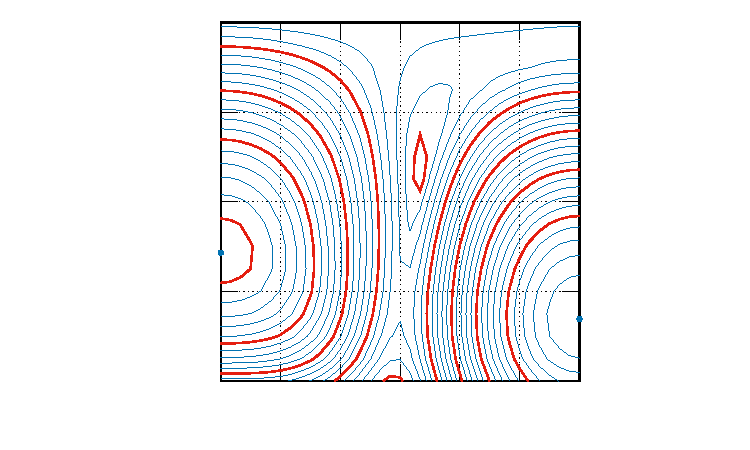
\includegraphics[width={360.00bp},height={216.00bp}]{figmapinvtorss0tot}}%
    \gplfronttext
  \end{picture}%
\endgroup
